\documentclass{beamer}

\usepackage[utf8]{inputenc}
\usepackage[T1]{fontenc}
\usepackage{amsmath}
\usepackage{bm}

\usepackage{tabularx}
\usepackage{graphicx}
\usepackage{epstopdf}
\usepackage{multirow}

\graphicspath{{../../images/}}

\usetheme{Madrid}
\usebeamercolor{sidebartab}
\usefonttheme{professionalfonts}


\title[M.Sc. Thesis 2015]{Spatial Summarization of Image Collections}
\author{Diego A. Ballesteros Villamizar}
\institute[ETHZ]{ETH Zürich}
\date{February 22nd, 2016}

\DeclareMathOperator*{\argmin}{argmin}
\DeclareMathOperator*{\argmax}{argmax}

\AtBeginSection[]
{
  \begin{frame}<beamer>
    \frametitle{Outline}
    \tableofcontents[currentsection]
  \end{frame}
}

\begin{document}

\begin{frame}
  \titlepage
\end{frame}

\section{Data and baseline model changes}

\begin{frame}{Clustering}
  \begin{itemize}
    \item A minor change on the mean-shift algorithm settings. "Orphan" photos are ignored, previously they were assigned to the closest cluster even if they were outside the bandwidth.
    \item This reduces the number of photos and paths in the dataset. E.g. For $N=10$ the number of paths is reduced from 8090 to 6781 and the number of photos covered is 30655. 
  \end{itemize}
\end{frame}

\begin{frame}{Markov model}
  \begin{itemize}
    \item Previously the Markov model had two issues: The set order was not preserved in the evaluation data and the model could use "future" items in the path for the prediction.
    \item After changes, the model is strictly as it would be used in an interactive system.
    \item To suggest an item given a partial sequence $S_{k}$, only the last item $s_{k}$ is used and the results are ordered according to the transition probabilities, i.e. $P(s_{k+1} = x \mid s_{k})$, learned from the data.
    \item The heuristic Markov model, assigns 0 probability to items previously seen in the path, i.e. $\forall_{x \in S_{k}} P(s_{k+1} = x \mid s_{k}) = 0$.
    \item This makes the model slightly worse than before, but still better than the current sub-/super-modular model.
  \end{itemize}
\end{frame}

\begin{frame}{Proximity model}
  \begin{itemize}
    \item Same as with the Markov model, the proximity model now only considers the items already seen in the path and only uses the distance from the item immediately before the one to predict in the sequence.
    \item This also decreases the accuracy score of the model.
    \item These changes allow the model to be used in a setting where a user is requesting item $k+1$ given a sequence $S_{k}$.
  \end{itemize}
\end{frame}

\section{Partial set size and scores}

\begin{frame}{Partial set size effect on score for $N=10$}
  \begin{figure}
    \centering
    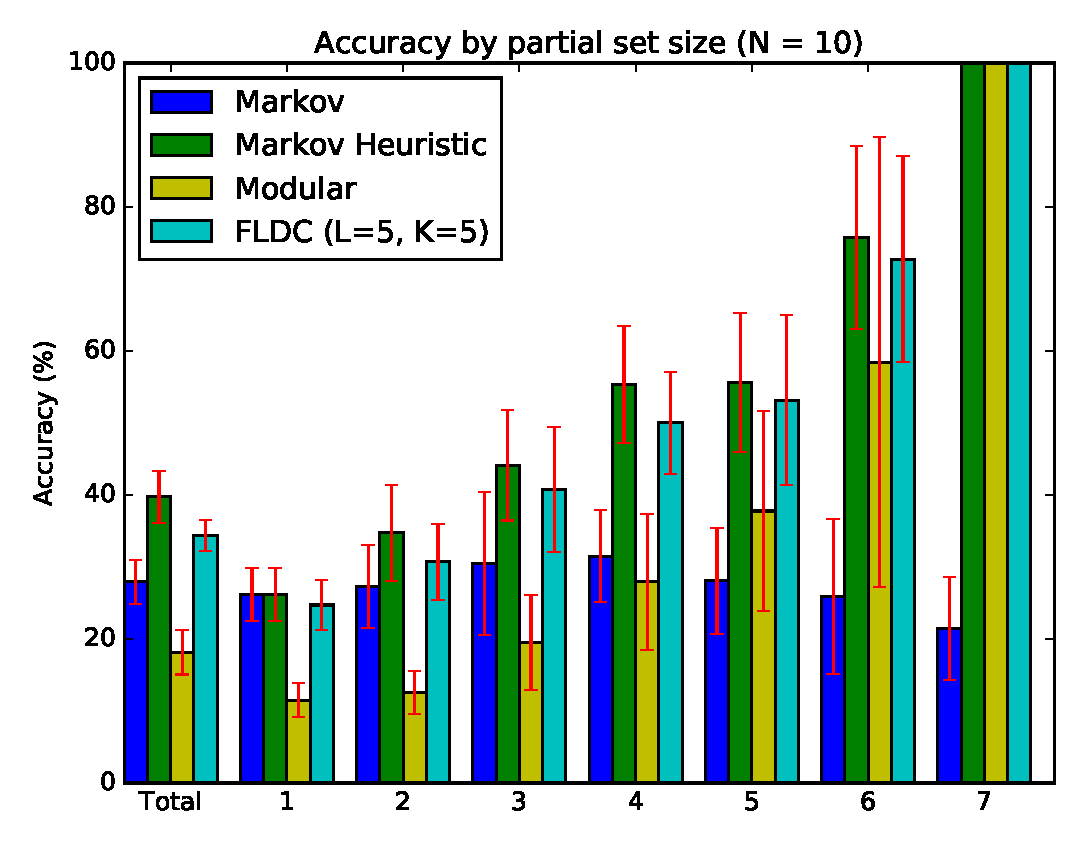
\includegraphics[width=0.8\textwidth]{set_size_score_10}
  \end{figure}
\end{frame}

\begin{frame}{Impact of heuristic methods}
  \begin{figure}
    \centering
    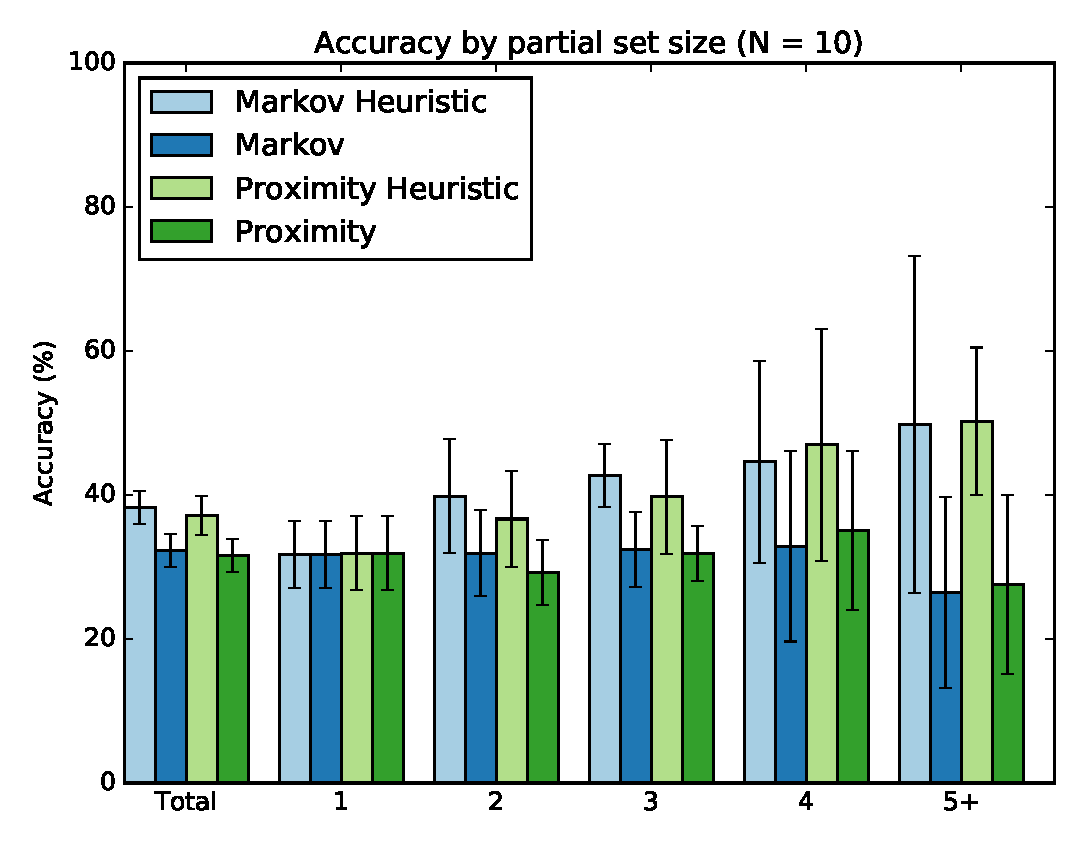
\includegraphics[width=0.8\textwidth]{set_size_score_10_heuristic_comparison}
  \end{figure}
\end{frame}


\begin{frame}{Partial set size effect on score for $N=50$}
  \begin{figure}
    \centering
    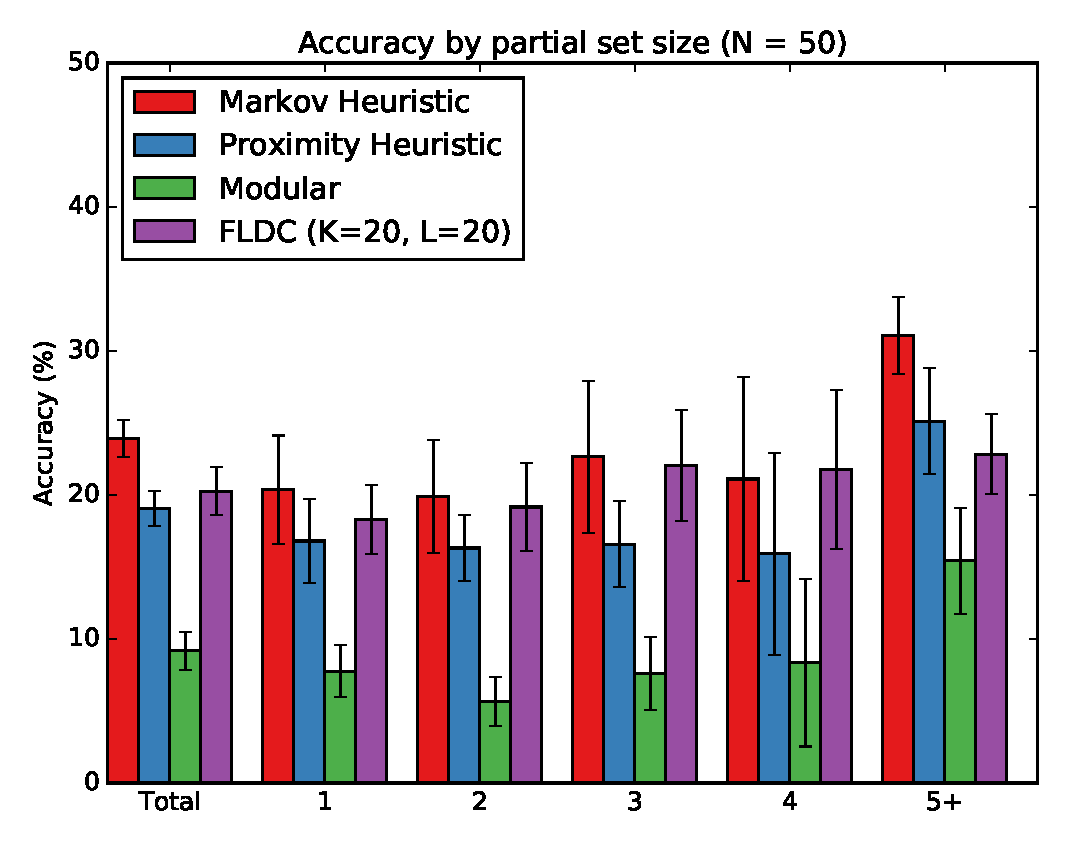
\includegraphics[width=0.8\textwidth]{set_size_score_50}
  \end{figure}
\end{frame}

\section{Changes in learning}

\begin{frame}{Learning from elements with at least 2 elements}
  \begin{itemize}
    \item A lot of the paths are singletons, which are not relevant to the evaluation and all methods except the modular one.
    \item Removing all singletons changes the dataset from 6781 to 1242 for $N=10$, and from 12614 to 2832 for $N=50$.
    \item The expectation is that singletons don't add relevant information when dealing with sets of 2 or more items.
    \item Markov and proximity models are not affected by this change, they already learn only from non-singleton paths.
  \end{itemize}
\end{frame}

\begin{frame}{Results comparison $N = 10$}
  \begin{figure}
    \centering
    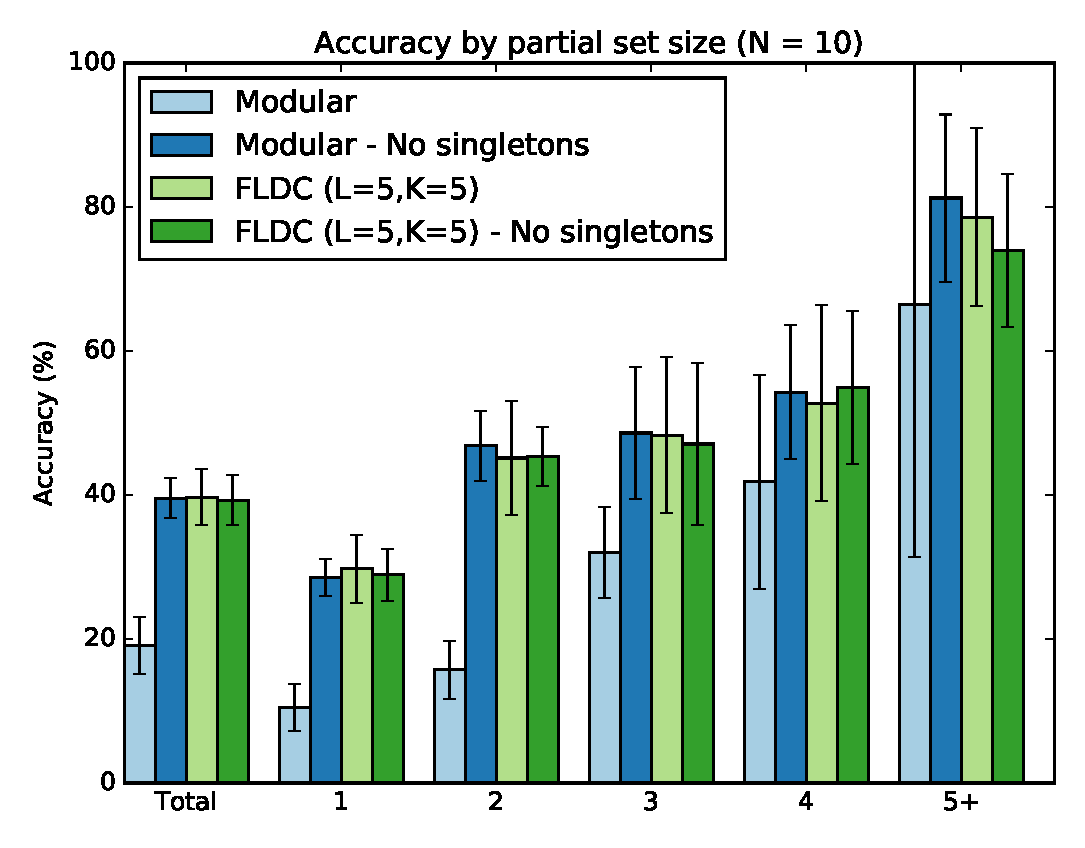
\includegraphics[width=0.8\textwidth]{set_size_score_10_no_singletons}
  \end{figure}
\end{frame}

\begin{frame}{Results comparison $N = 50$}
  \begin{figure}
    \centering
    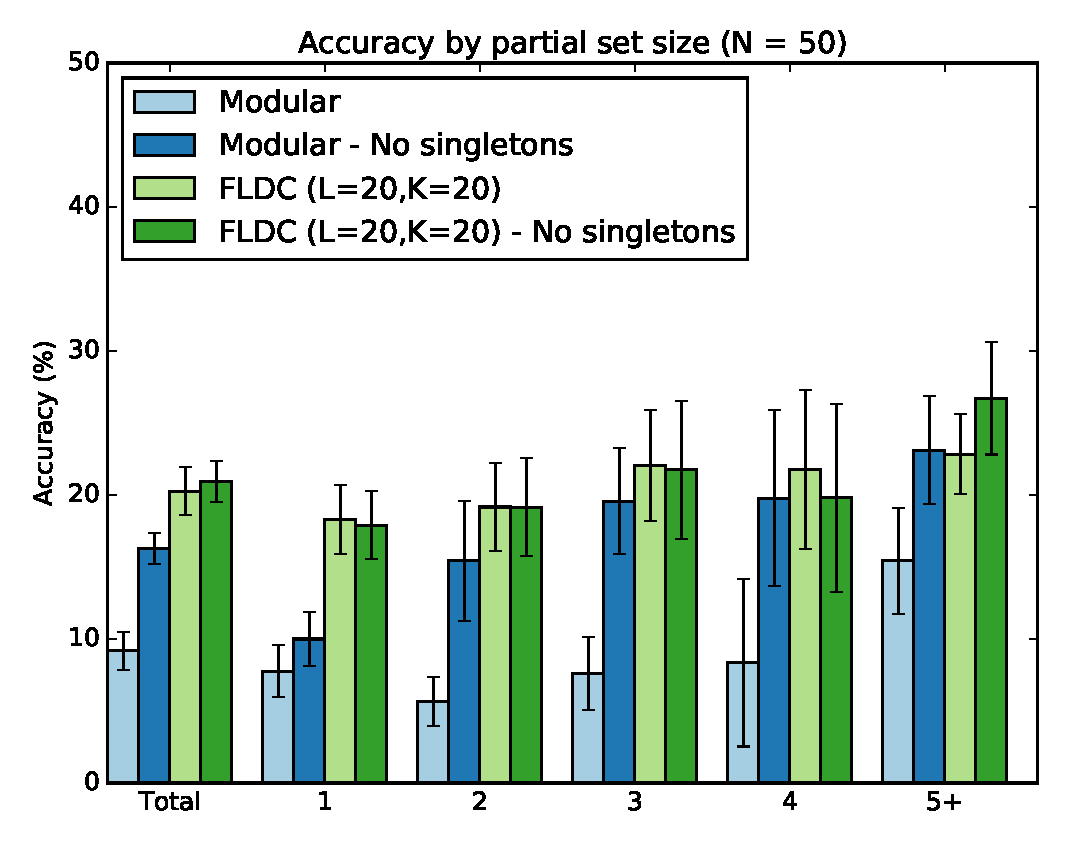
\includegraphics[width=0.8\textwidth]{set_size_score_50_no_singletons}
  \end{figure}
\end{frame}

\begin{frame}{Results comparison $N = 100$}
  \begin{figure}
    \centering
    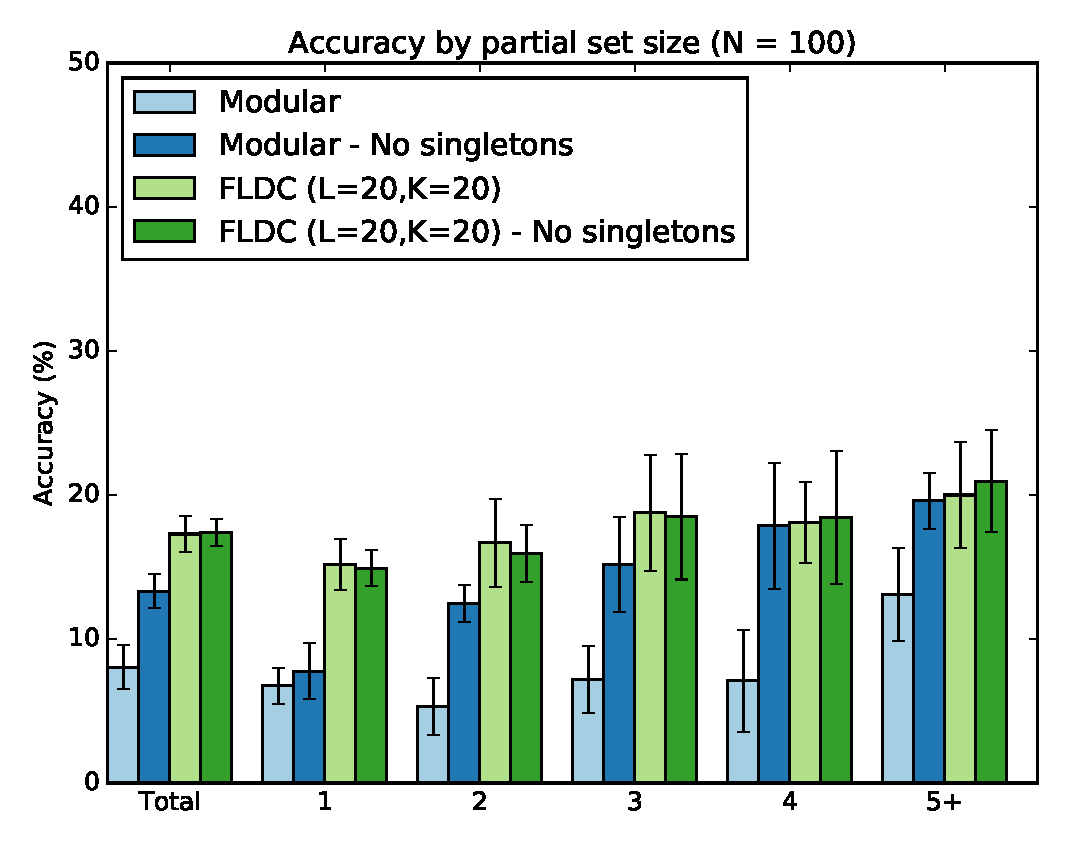
\includegraphics[width=0.8\textwidth]{set_size_score_100_no_singletons}
  \end{figure}
\end{frame}

\section{Data distribution and sampling}

\begin{frame}{Set size distribution in data}
  \begin{figure}
    \centering
    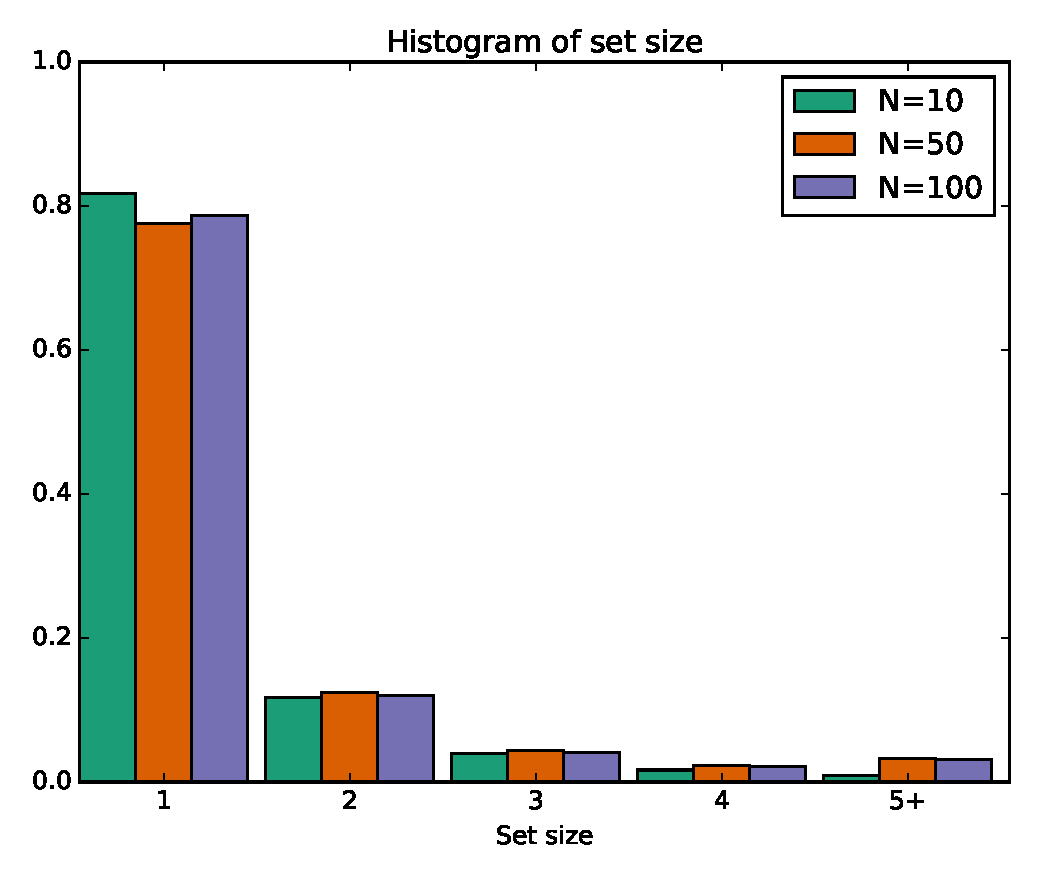
\includegraphics[height=0.8\textheight]{data_size_histogram}
  \end{figure}
\end{frame}

\begin{frame}{Set size distribution after sampling}
  \begin{figure}
    \centering
    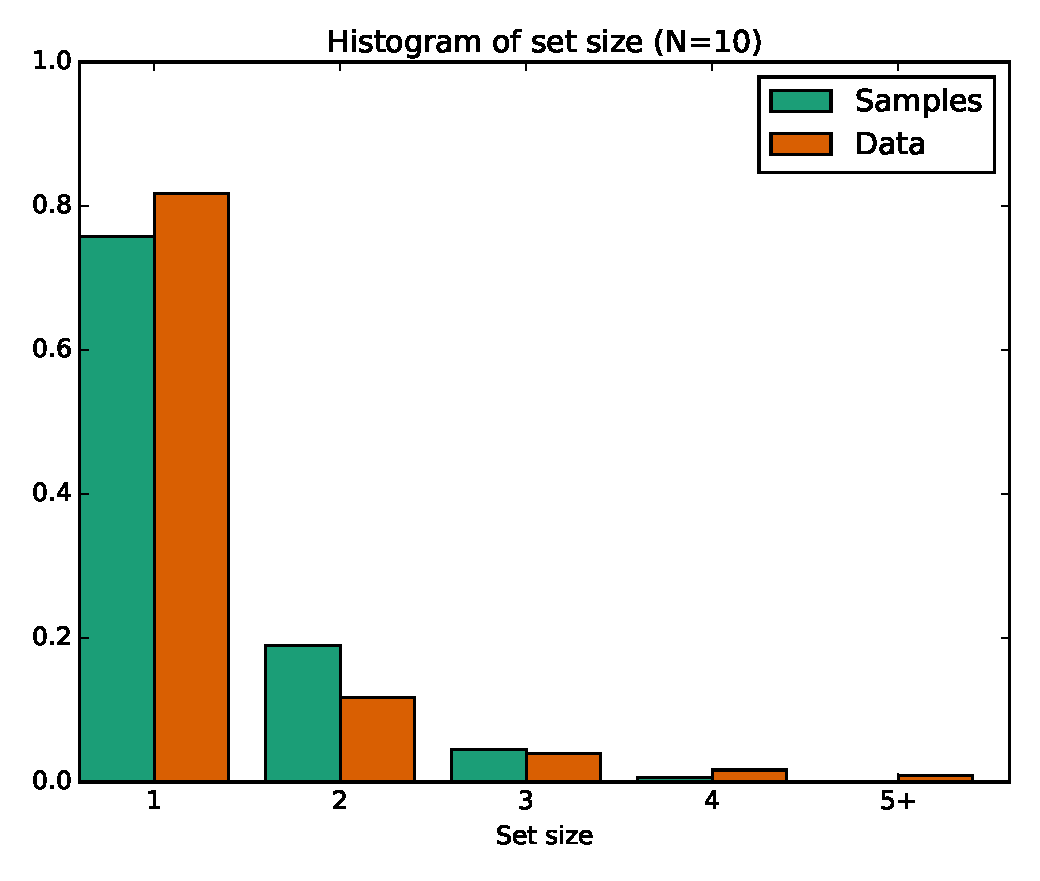
\includegraphics[height=0.8\textheight]{data_sampling_histogram_10_with_singletons}
  \end{figure}
\end{frame}

\begin{frame}{Set size distribution after sampling - no singletons}
  \begin{figure}
    \centering
    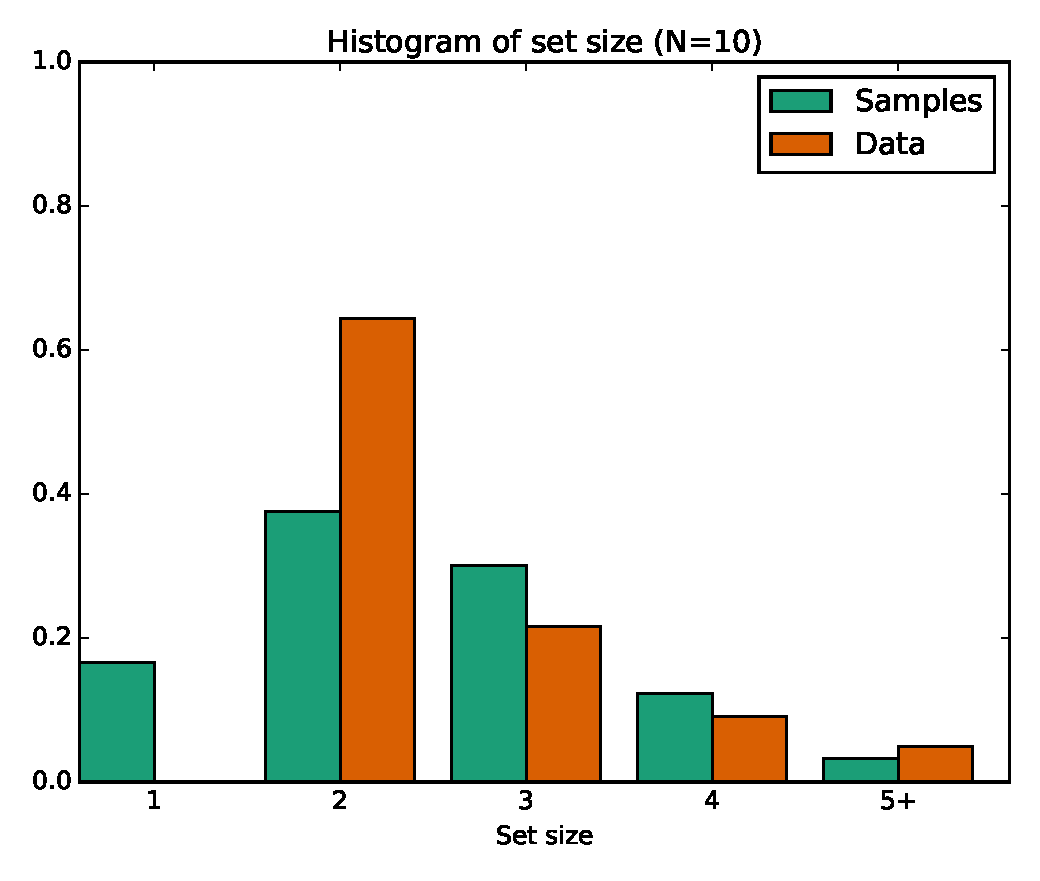
\includegraphics[height=0.8\textheight]{data_sampling_histogram_10}
  \end{figure}
\end{frame}

\section{Featurized models}

\begin{frame}{Dataset creation}
  \begin{itemize}
    \item First remove "duplicates", i.e. photos with the exact same location.
    \item Filter photos that do not form a path of more than one item, i.e. when a user takes a single photo in a day.
    \item Sample 10k photos from the resulting set.
    \item Form a path dataset from the sample and remove singleton paths.
    \item The result has 1936 paths and comprises 9141 photos.
  \end{itemize}
\end{frame}

\begin{frame}{Feature definition}
  \begin{itemize}
    \item Ten reference points corresponding to the top 10 cluster centers calculated using mean-shift clustering.
    \item For each item, the feature vector contains the distances to each cluster center.
    \item $\mathbf{X} \in \mathbb{R}^{9141 \times 10}$.
  \end{itemize}
\end{frame}

\begin{frame}{Models}
  \begin{itemize}
    \item A baseline proximity model that proposes an item closest to the previous item in the sequence.
    \item Modular model that using frequencies computes the utility vector $\mathbf{u} \in \mathbb{R}^{10}$.
    \item FLDC model with features, dimension parameters $L=10, K=10$.
    \item The results are:
    
    \begin{table}
      \centering
      \begin{tabular}{@{}ll@{}}
        \hline
        \textbf{Model} & \textbf{MRR (\%)}\\
        \hline
        Proximity & $18.94 \pm 3.28$ \\
        Modular & $0.11 \pm 0.04$ \\
        FFLDC (L=10, K=10) & $0.10 \pm 0.04$ \\
        FFLDC (L=20, K=20) & $0.07 \pm 0.03$ \\
        \hline
      \end{tabular}
    \end{table}
  \end{itemize}
\end{frame}

\begin{frame}{Bad model?}
  \begin{itemize}
    \item Another possible dataset to test the featurized model is the dataset of all mean-shift clusters without filtering the top N.
    \item Feature vector is the location of each cluster center.
    \item Dataset has 6431 paths with more than one element, out of 27707, and 2685 items.
  \end{itemize}
\end{frame}

\begin{frame}{Evaluation}
  \begin{figure}
    \centering
    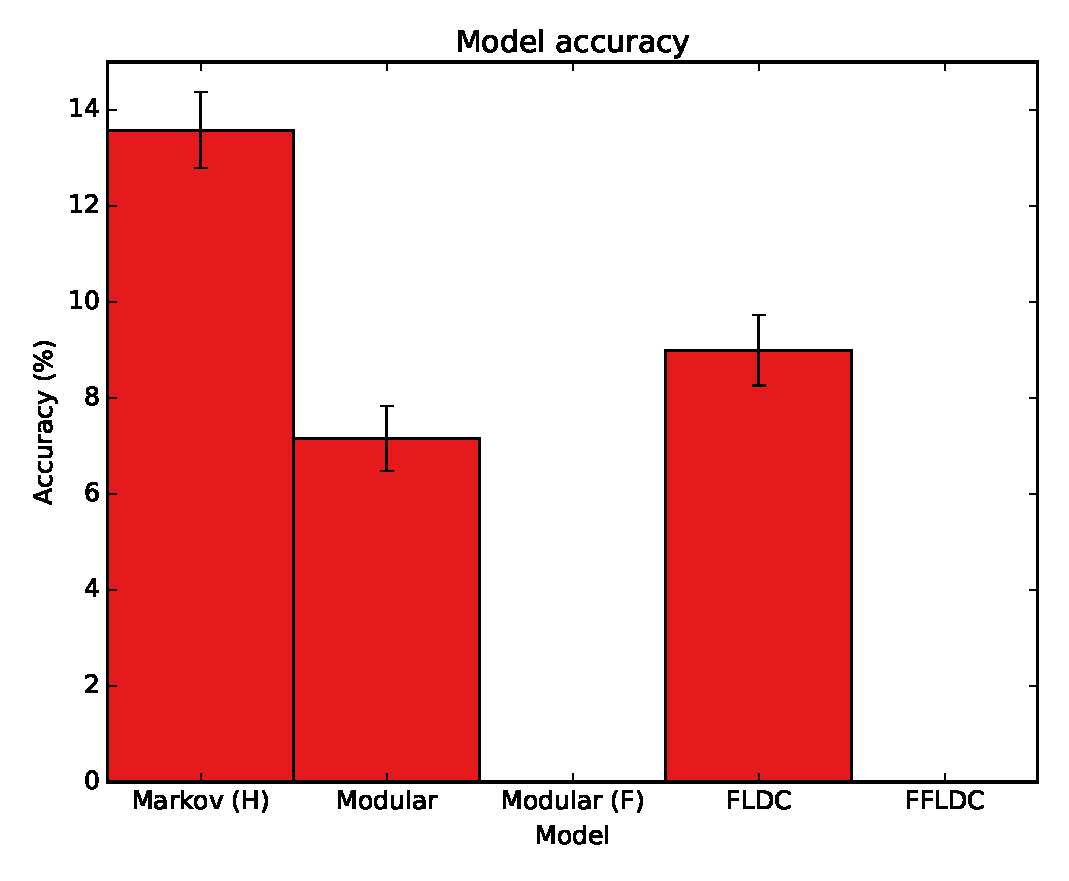
\includegraphics[height=0.8\textheight]{score_all}
  \end{figure}
\end{frame}


%\begin{frame}{References}
%  \bibliographystyle{acm}
%  \bibliography{../references}
%\end{frame}

\end{document}
